\mychapter{Projeto SpaceVANT}
\label{Cap:SpaceVANT}

O projeto SpaceVANT é um projeto desenvolvido pela Universidade Federal do Rio Grande do Norte (UFRN), alocado no Departamento de Engenharia da Computação e Automação, em parceria com o Centro de Lançamento Barreira do Inferno (CLBI). O projeto tem por objetivo tornar o processo de verificação da área de impacto de foguetes lançados pelo CLBI mais eficiente tanto em relação ao tempo gasto quanto ao custo financeiro.

\section{Solução Atual}

Atualmente, a área provável de impacto de um foguete a ser lançado é vistoriada com o auxílio de um avião tripulado que sobrevoa a área em busca de embarcações não autorizadas. Somente quando o avião sobrevoa toda a região e certifica que nenhum embarcação se encontra no local, o lançamento poderá ser autorizado.

A solução empregada no momento possui alguns pontos negativos, primeiramente, o custo com os aviões que realizarão a operação de varredura, bem como o custo de manutenção dos mesmo, é bastante elevado quando comparado com o custo de aquisição e manutenção de VANTs. Além disso, os aviões utilizados, atualmente, para fazer o processo de varredura, bem como os pilotos, são cedidos pela base aérea de Natal, o que gera um dependência de recurso externo ao CLBI podendo atrasar a operação de lançamento de foguetes devido a indisponibilidade de aviões e pilotos por parte da base aérea. 

\section{Objetivo do Projeto}


No intuito solucionar o problema apresentado de forma mais eficaz, o projeto SpaceVANT visa desenvolver sistema de VANTs autónomos que irá realizar a varredura da área de impacto. O produto final do projeto incluirá: sistema supervisório, estação base, aeronaves autónomas do modelo \emph{Penguin} (Fig \ref{fig:penguin}) dotadas de computador e câmera fotográfica embarcados, sistema de processamento de imagens e, por fim, uma rede de comunicação que conectará todas a aeronaves e a estação base. 

\begin{figure} 
\center
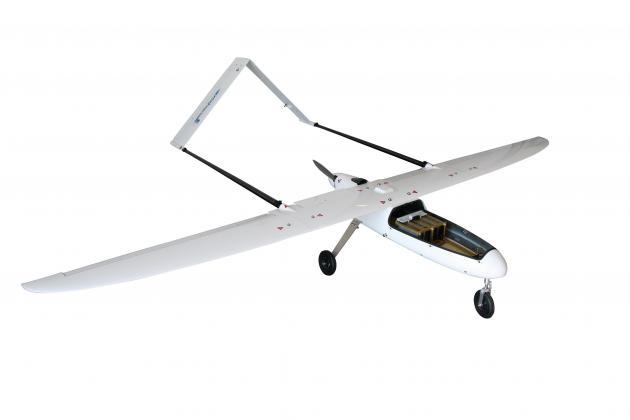
\includegraphics[width=0.7\textwidth]{penguin.jpg}
\caption{Aeronave modelo Penguin.} 
\label{fig:penguin}
\end{figure}

Para a realização da missão de varredura serão necessárias algumas entradas ao sistema, sendo elas, a quantidade de aeronaves a serem empregadas na missão, tempo de duração da missão, área a ser varrida e estratégia de varredura a ser utilizada, estratégias essas que serão apresentadas no Cap. \ref{Cap:Estrategia}.

Quando fornecidas todas as entradas corretamente, as rotas de voo serão definidas e carregadas nos VANTs e a missão terá inicio. O progresso da missão poderá ser acompanhado através da estação base e, caso alguma embarcação seja identificada, um alerta será lançado pela rede até chegar a estação base alertando o operador da missão. Esse alerta será composto pela imagem da possível embarcação identificada pelo sistema, a localização geográfica do objeto e a hora na qual ele foi identificado.\\  

Dado o contexto em que esse trabalho se encontra e o objetivo do projeto SpaceVANT, as características de um rede multi VANTs para a aplicação serão discutidas a seguir.





 